\section{Hyperparameter Tuning}
\subsection{Grid Search}
Grid Search, bir makine öğrenme modelinin hiperparametrelerini ayarlamak için kullanılan bir hiperparametre tuning yöntemidir. Bu yöntem, belirli bir hiperparametre uzayında tüm olası kombinasyonları deneyerek en iyi hiperparametre setini bulmayı amaçlar. Grid Search, parametrelerin bir ızgara gibi düzenlendiği ve her hiperparametre kombinasyonunun denendiği bir arama sürecini içerir.

\begin{figure}[h]
    \centering
    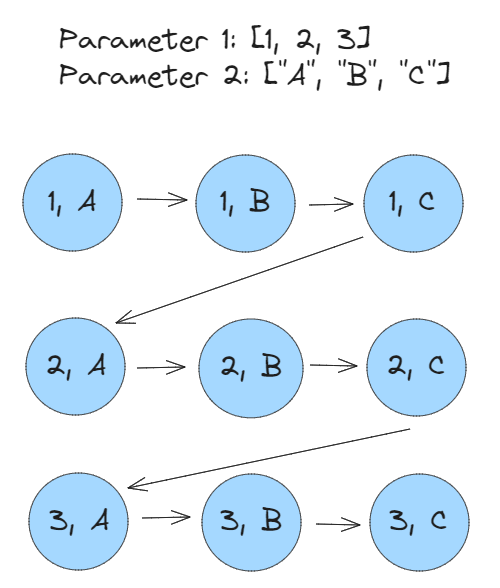
\includegraphics[width=0.5\textwidth]{images/Grid_Search.png}
    \caption{Izgara araması.}
    \label{fig:enter-label}
\end{figure}

\subsubsection{Avantajları}
\begin{enumerate}
    \item Tüm hiperparametre kombinasyonlarını denediği için en iyi sonuçları elde etme olasılığı yüksektir.
    \item Basit ve anlaşılır bir yaklaşım, hiperparametrelerin aralığını ve adım büyüklüğünü belirlemek kolaydır.
    \item Özellikle küçük veri setleri için etkili olabilir.
\end{enumerate}

\subsubsection{Dezavantajları}
\begin{enumerate}
    \item Hesaplama maliyeti yüksektir, çünkü tüm kombinasyonlar denendiğinden, büyük veri setlerinde veya çok sayıda hiperparametrele sahip modellerde kullanmak zaman alabilir.
    \item İzgara araması, hiperparametreler arasındaki etkileşimleri dikkate almaz.
    \item Optimum hiperparametrelerin belirlenmesi için birçok deneme gerekebilir.
\end{enumerate}

\begin{lstlisting}[language=Python]
from sklearn.model_selection import GridSearchCV
from sklearn.svm import SVC

# Hiperparametreler ve deger araliklari
param_grid = {'C': [0.1, 1, 10], 'kernel': ['linear', 'rbf']}

# Model
svm_model = SVC()

# Grid Search
grid_search = GridSearchCV(estimator=svm_model, param_grid=param_grid, cv=5, scoring='accuracy')
grid_search.fit(X_train, y_train)

# En iyi hiperparametre kombinasyonu ve sonuc
best_params = grid_search.best_params_
best_score = grid_search.best_score_

print("En iyi hiperparametreler:", best_params)
print("En iyi dogruluk:", best_score)
\end{lstlisting}

\newpage

\subsection{Random Search}
Random Search, hiperparametre tuning yöntemlerinden biridir ve makine öğrenme modellerinin hiperparametrelerini ayarlamak için kullanılır. Random Search, Grid Search gibi tüm hiperparametre kombinasyonlarını denemek yerine rastgele seçilen hiperparametre kombinasyonlarını kullanarak modelin performansını değerlendirir. Bu yöntem daha verimli olabilir ve daha iyi sonuçlar elde etme olasılığı yüksektir.

\begin{figure}[h]
    \centering
    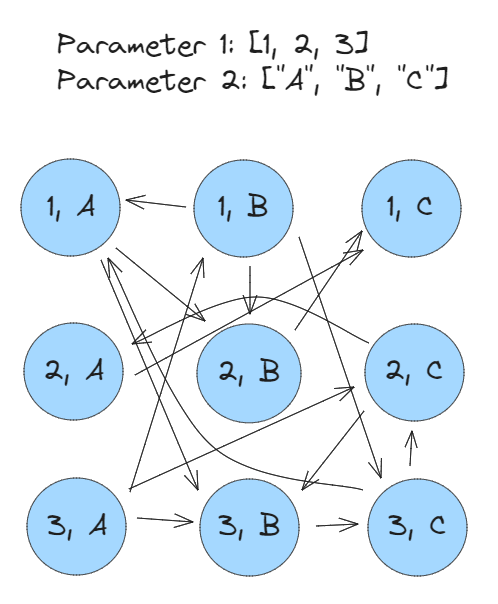
\includegraphics[width=0.5\textwidth]{images/Random_Search.png}
    \caption{Rastgele arama.}
    \label{fig:enter-label}
\end{figure}

\subsubsection{Avantajları}
\begin{enumerate}
    \item Hesaplama maliyeti, Grid Search'e göre genellikle daha düşüktür, çünkü rastgele kombinasyonlar denendiğinden daha az model eğitilir.
    \item Optimum hiperparametreleri belirleme olasılığı Grid Search'e göre daha hızlıdır, özellikle büyük hiperparametre uzaylarında.
\end{enumerate}

\subsubsection{Dezavantajları}
\begin{enumerate}
    \item En iyi sonuçları elde etmek için daha fazla denemeye ihtiyaç duyabilir, çünkü rastgele kombinasyonlar şansa bağlıdır.
    \item Hiperparametreler arasındaki etkileşimleri yakalamak zor olabilir, çünkü rastgele seçilen kombinasyonlar arasında bu etkileşimler olmayabilir.
\end{enumerate}

\begin{lstlisting}[language=Python]
from sklearn.model_selection import RandomizedSearchCV
from sklearn.svm import SVC
from scipy.stats import uniform, randint

# Hiperparametreler ve deger araliklari
param_dist = {
    'C': uniform(loc=0.1, scale=9.9),
    'kernel': ['linear', 'rbf']
}

# Model
svm_model = SVC()

# Random Search
random_search = RandomizedSearchCV(estimator=svm_model, param_distributions=param_dist, n_iter=10, cv=5, scoring='accuracy')
random_search.fit(X_train, y_train)

# En iyi hiperparametre kombinasyonu ve sonuc
best_params = random_search.best_params_
best_score = random_search.best_score_

print("En iyi hiperparametreler:", best_params)
print("En iyi dogruluk:", best_score)
\end{lstlisting}

\subsection{Particle Swarm Optimization (PSO)}
PSO (Particle Swarm Optimization), kuş sürülerinin ve bal arılarının davranışlarından esinlenen bir evrimsel optimizasyon algoritmasıdır.
PSO, birçok olası çözüm noktasını temsil eden parçacıkların birbirleriyle etkileşimde bulunarak, bir hedef işlevi en iyilemek için bir araya gelmesini simüle eder.

\subsection{Genetic Algorithm (GA)}
Genetik Algoritma (Genetic Algorithm - GA), biyolojik evrim süreçlerinden esinlenen bir evrimsel optimizasyon tekniğidir. 
Genetik algoritma, çözüm uzayında potansiyel çözümleri genetik operatörler (çaprazlama, mutasyon, seçilim) kullanarak geliştirir 
ve bu operatörler yoluyla en iyi çözümü bulmaya çalışır. 

\subsection{Optuna}
Optuna, en iyi parametre setini bulmak için parametrelerin rastgele kombinasyonlarını deneyen bir yöntemdir. GridSearch'e ve RandomSearch'e göre daha hızlı çalışabilir. Ayrıca, parametreler arasındaki ilişkileri dikkate alarak daha iyi parametre kombinasyonları bulur. Bayesian Optimization yöntemi kullanılarak gerçekleştirilir.

\begin{lstlisting}[language=Python]
import optuna
from sklearn.datasets import load_iris
from sklearn.model_selection import train_test_split
from sklearn.tree import DecisionTreeClassifier

# Veriyi yukle
data = load_iris()
X, y = data.data, data.target

# Egitim ve test veri setlerini olustur
X_train, X_test, y_train, y_test = train_test_split(X, y, test_size=0.2, random_state=42)

# Optuna ile optimize edilecek hiperparametreleri tanimla
def objective(trial):
    # Hiperparametreler
    max_depth = trial.suggest_int("max_depth", 1, 32)
    min_samples_split = trial.suggest_float("min_samples_split", 0.1, 1.0)
    min_samples_leaf = trial.suggest_float("min_samples_leaf", 0.1, 0.5)

    # Karar agaci modelini olustur
    model = DecisionTreeClassifier(
        max_depth=max_depth,
        min_samples_split=min_samples_split,
        min_samples_leaf=min_samples_leaf,
    )

    # Modeli egit ve dogruluk skoru hesapla
    model.fit(X_train, y_train)
    accuracy = model.score(X_test, y_test)
    return accuracy

# Optuna calistir
study = optuna.create_study(direction="maximize")  # Maksimize edilen metrik (dogruluk)
study.optimize(objective, n_trials=100)  # 100 farkli deneme yap

# En iyi hiperparametreleri ve sonucu al
best_params = study.best_params
best_accuracy = study.best_value

print("En iyi hiperparametreler:", best_params)
print("En iyi dogruluk:", best_accuracy)
\end{lstlisting}

\newpage